\subsection{ZFS 特点}
\subsubsection{Unified Storage}
从IT管理角度,
ZFS 重大特色在于其提供统一的存储系统,
既提供文件系统服务,也提供块设备接口,
即兼具了NAS和SAN的功能,
统一存储系统使得部署和管理存储系统得到简化。

\subsubsection{Data Integrity}
ZFS 的设计最重要关注点是保护数据的完整性,
为实现这个目标,
ZFS 对所有的数据块都计算较验和,
并把较验和存储于用于寻址该数据快的快指针内,
即每个子节点的较验和存于其父节点处。

\subsubsection{Copy-On-Write}
ZFS 的另一大特色在于其数据写入方式。
和常见文件系统采用的块内直接修改不同,
ZFS 采用 COW({\em Copy-On-Write})%
\footnote{不做块内修改的思路来自{Log Structured Filesystem}}
机制写入永久存储介质。
COW 的效果就是直至修改文件系统组织树的根(即,Uberblock)之前,
所做的改动不可见并且源树不会遭到任何修改,
这期间掉电或崩溃不影响源树。
图\,\ref{fig:cow}\,展示了写入某些块的COW过程。

\begin{figure}[!ht]
  \centering
  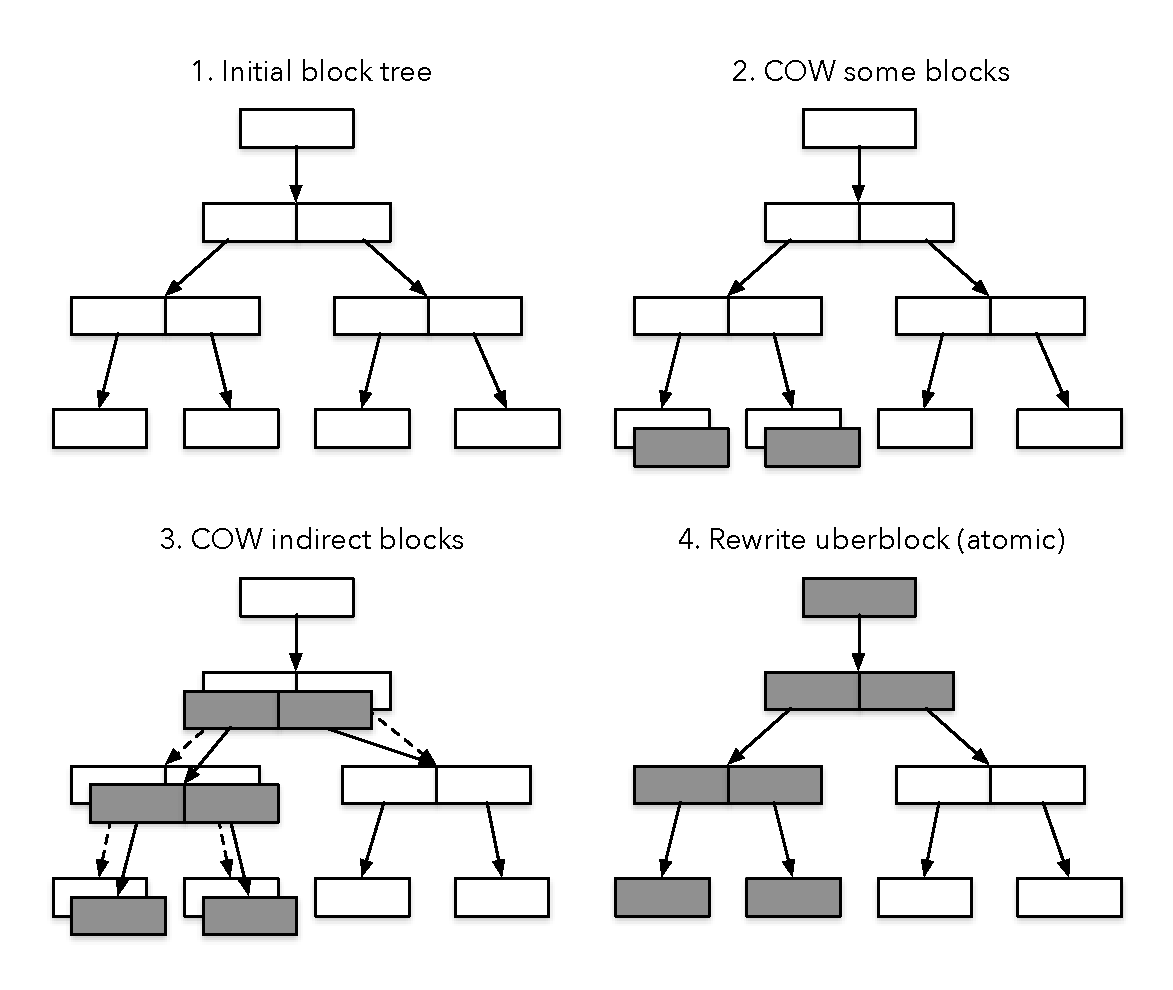
\includegraphics[width=\textwidth]{fig/zfs_cow.pdf}
  \caption{COW}\label{fig:cow}
\end{figure}

传统文件系统当掉电或系统崩溃后极容易出现\emph{文件系统}不一致。
导致不一致问题的本质原因是文件系统的数据更新涉及一系列文件系统内部结构的改动。
譬如对某个文件尾部追加一个数据块,
至少以下的几个步骤要完成:
\begin{enumerate*}[label=\itshape\alph*\upshape)]
  \item 分配一个数据块并写入该数据块;
  \item 修改维护块分配状况的数据结构,位图或B-树等;
  \item 文件的{\em inode}也需要更新,文件长度、修改时间等属性,数据块寻址数据结构。
\end{enumerate*}
这一系列改动可能部分成功部分失败,
并且不保证各部分更新的顺序。
可能有以下几种情况:
\begin{itemize}
  \item 只有数据块分配和写入成功,
    这不是问题,仅仅是刚写入的数据丢失,
    文件系统压根就不知道有这么个数据块存在过;
  \item 只有对inode的更新成功,
    这个后果就严重了,
    \begin{enumerate*}[label=\itshape\alph*\upshape)]
      \item 数据块的指针已写入,而数据未完成,于是从该指针处读出的是垃圾数据
      \item 文件系统的块管理部分未更新,而inode指出某个地址上的块有数据,
        出现文件系统不一致问题;
    \end{enumerate*}
  \item 只有块管理部分得到更新,块管理声明某个块已分配,不能挪作它用,
    但文件系统其它部分又没有使用到它,这称为空间泄漏;
  \item 块管理和inode成功更新而数据未写入,文件系统一致,但用户将得到垃圾数据;
  \item inode和数据写入而块管理未更新,文件系统不一致;
  \item 块管理和数据写入而inode未更新,空间泄漏。
\end{itemize}

传统文件系统通过{\em fsck}工具来解决不一致问题。
\begin{itemize}
  \item fsck从超级块开始,
    检查其正确性,
    如果需要从已知健全的备份超级块恢复;
  \item 而后fsck扫描所有的inode,
    数据块指针,间接快指针,根据它们判断那些块已分配,
    如果和块管理不一致,以inode为准修改块管理数据结构;
  \item fsck试图修正inode的状态,譬如文件类型等属性,
    如果发现inode无法被修正,该inode被丢弃,
    并相应修改块管理数据结构与之匹配;
  \item 修复inode和目录之间链接,
    这通过从根目录开始扫描所有的目录,计算哪些目录项链接到某个inode,
    如果数目不一致,通常修正inode中的链接数;
  \item 一旦发现有多个块指针指向同一块地址,
    如果其中有明显错误,fsck丢弃该块指针,
    否则fsck创建数据块的拷贝,使每个块指针指向自己独享的块;
  \item fsck检查块指针是否合法,譬如其是否指向硬盘分区之外的地址,
    如果块指针被发现不合法,
    fsck能做的最好处理就是从inode或间接指针中删除它;
  \item fsck也修正目录的内容,
    譬如目录``.''和``..''必须是一个目录的头两个目录项
\end{itemize}
可想而知,
fsck的全文件系统扫描机制非常低效。
现代的文件系统引入日志 ({\em journal}) 的概念,
即对文件系统改动之前,
将对更新全过程精确描述先写入存储介质,
当更新过程被意外中断重启系统或重新挂载文件系统时,
可以通过该日志知晓出了什么问题以及如何修复。
一个立刻浮现的问题是,
日志的内容可能很大,
如何保证日志本身的完整性?
答案是只能靠硬件保证。
\footnote{
  题外话,
  现代硬盘不保证多个写入请求按收到的顺序完成,
  即便使用写屏障({\em Write Barrier}) 也有可能被硬件忽略。
}
现代硬盘通常保证一次512字节写入的原子性,
于是日志写入分为两阶段,
\begin{enumerate}
  \item 日志写入,
    即先将日志开始标志和日志内容先写入,这一阶段的原子性无法保证,
    内容写入成功之后,文件系统:
  \item 将日志结束标志原子地写入磁盘
\end{enumerate}
这样一来,日志的完整与否可以由日志结束标志判定。
Linux的Ext4文件系统通过使用较验和实现对日志的一次性写入而不失完整性,
提高了日志写入的效率。
日志文件系统的缺点是任何数据写都要对磁盘操作两次。

回到ZFS,
正因为数据的COW语义,
没有就地修改的数据块,
意外断电或系统崩溃的恶果仅仅是丢失部分未写入数据,
文件系统的一致性得到保障而无需做fsck或日志回放。

\subsubsection{Snapshot \& Clone}
得益于Copy-On-Write机制,
ZFS提供高效的快照({\em Snapshot})和克隆({\em Clone})功能。
对文件系统创建快照之后,
当写入原始文件系统发生COW,
旧数据不会被回收使用,
旧的数据块树将一直存在,
部分新数据和旧数据组成一棵新树,
呈现一个新文件系统。
克隆即可写快照,
所有内容没有被修改过的数据块被共享,
写入克隆文件系统只是导致树产生分杈而不是全部复制。

ZFS文件系统可以被移入另外一个存储池中,
更进一步,
可以被发送到远程。
send命令创建一个流呈现文件系统的状态,
这个流可以呈现某个快照的所有内容,
也可以是两个快照之间的增量,
这提供了一个高效的策略,
用于譬如在HA中同步存储池或者将存储备份至其它主机。

\subsubsection{Transactional Model}
写入请求被归入某个终将写入存储池的事务组中,
事务的含义就是写入以组为原子单位,
ZFS的DMU层不允许部分成功部分失败的情形。
每一个事务组对应文件系统一个一致的状态({\em checkpoint}),
事务组完全写入磁盘后,
即一个checkpoint产生之后,
对uberblock进行一次原子写,
更新事务组号,
于是文件系统跃迁至一个新的、一致的状态上。

\subsubsection{其它}
ZFS还提供数据压缩,加密等用户需要的功能。

ZFS 另外有几个先进的实现,
\begin{description}
  \item[ARC, {\em Adaptive Replacement Cache}]\hfill\\
    ARC 是一个物理页管理算法,效率高于传统的 LRU。
    本质上说 ARC 除了考虑页的使用时间点之外还考虑页的使用频率,
    当需要回收页时,
    ARC算法有效决定从LRU还是LFU链表中选取,
    并动态、自适应地决定两条链的长度。
    除了位于内存中的缓存,
    ZFS引入了二级缓存 ({\em L2ARC}) 的概念,
    将一大部分页缓存放在SSD上免去某些页被换出后需要再次读取而操作磁盘;
  \item[ZIO pipeline]\hfill\\
    将I/O分为20道工序,
    按流水线方式处理,
    使得I/O不同阶段的工序可以在不同的CPU核上完成,
    充分利用多核CPU并行运算能力从而提高吞吐量;
  \item[Space Map]\hfill\\
    实现高效分配、释放存储设备上的块。
\end{description}

\subsubsection{缺点}
COW 的优点是集中了分散的写,
如写不同文件的数据,
又如文件的数据写伴随metadata的写\footnote{数据和元数据往往距离较远},
使它们成为线性写,
大大提高写效率。
但是这产生一个副作用,
文件相邻的块物理上可能非常分散,
造成读效率较低,
这个只能通过大内存做cache和好的缓存算法来适当抵消。

COW 另外一个缺点是会导致碎片,
在磁盘使用率超过70\%,
所有的metaslab都已创建,
其中都或多或少被填充,
文件写入将出现性能瓶颈,
IOPS下降较严重。

\subsection{ZFS组织结构}
一个存储池{\em zpool}是由虚拟设备{\em vdev}节点构成的一棵树。
位于叶端的是负责实际数据存取的物理介质,
故称为{\em phsical vdev};
其余的节点统称为{\em logical vdev},
用于表示 ZFS 的逻辑。
ZFS 藉由抽象的虚拟设备树即可实现不同的Raid级别。

\begin{figure}[ht]
  \centering
  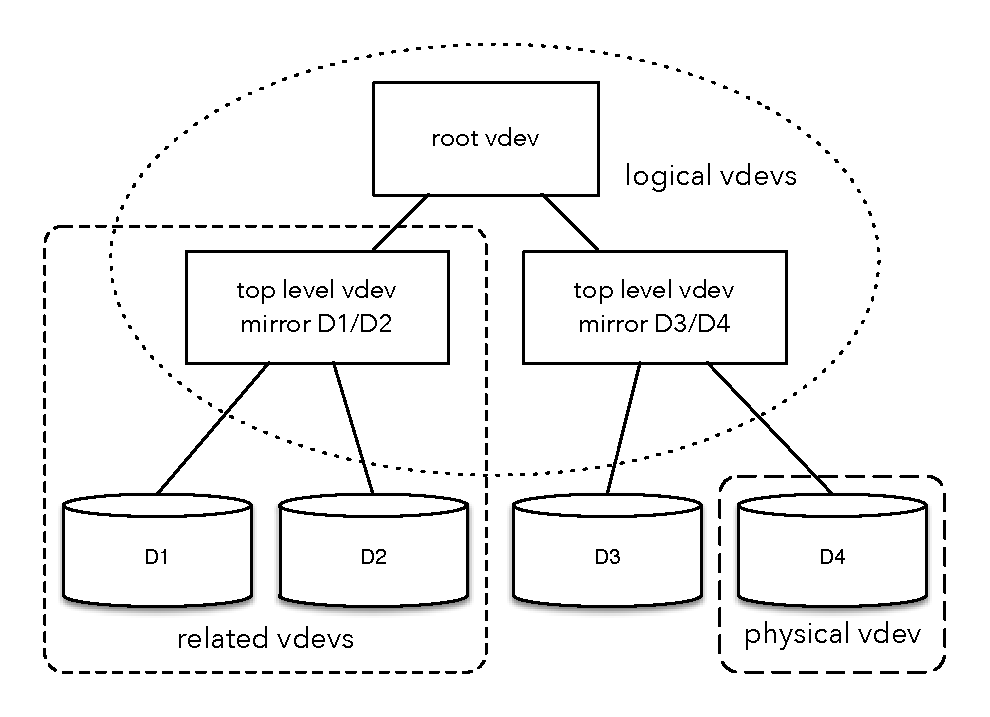
\includegraphics[width=\textwidth]{fig/zfs_architecture.pdf}
  \caption{ZFS架构}\label{fig:arch}
\end{figure}

图\,\ref{fig:arch}\,所表示的存储池结构由如下命令创建,
第二个 mirror 关键字表示将指定新的顶层虚拟设备。
数据通过这两个镜像以动态方式进行条带化,
并会相应地在每个磁盘之间创建冗余数据。
\begin{lstlisting}{lanuage=Bash}
# zpool create tank mirror D1 D2 mirror D3 D4
\end{lstlisting}

\subsection{ZFS代码模块}
从设计实现的角度看,
ZFS 分为 7 个相对独立模块,
模块的简称贯穿整个ZFS文件系统的代码及文档之中。

\begin{description}
  \item[SPL, {\em Storage Pool Allocator}\,:]
    负责存储池一级的操作,如创建,销毁,修改属性等;
  \item[DMU, {\em Data Management Layer}\,:]
    完成将数据块组织为对象,如文件、目录等,
    并且将对象组织为对象集,如文件系统、文件系统快照等;
  \item[DSL, {\em Dataset and Snapshot Layer}:]
    管理对象集属性以及各对象集之间逻辑关系
  \item[ZAP, {\em ZFS Attribute Processor}\,:]
    位于 DMU 层之上,
    操作称为 ZAP 的对象,
    ZAP 对象用于描述如文件系统、存储池等对象集的属性;
  \item[ZPL, {\em ZFS Posix Layer}\,:]
    将 ZFS 的对象、对象集以 Posix 标准的方式呈现,
    提供 POSIX 标准方式的文件操作,如 open、read、write;
  \item[ZIL, {\em ZFS Intent Log}\,:]
    ZIL 保存来自系统调用的写操作的纪录,
    描述写操作本身的数据量比为维护文件系统一致性%
    而引发的一连串写要小多了。
    ZIL 用于当系统崩溃或意外掉电时回放该事务,
    可找回部分数据。
    启动一个 DMU 事务同时会启动一个 ZIL 事务,
    并在 {\em fsync}%
    \footnote{{\em fsync}的语义就要求写入被从内存中刷到永久存储介质上}
    时被写入永久存储设备。
    但此时文件系统的checkpoint还未真正完成,
    如果此时掉电或系统崩溃,
    文件系统仍处于之前一个一致的checkpoint,
    这种情况就可以通过对ZIL的{\em reclaim}来追回数据。
    当该 DMU 事务成功完成之后,
    因为一个一致的checkpoint已经产生,
    之前写操作的 ZIL 可以丢弃;
    通常采用一个快速 SSD 专门用于 ZIL 存储设备提高效率;
  \item[ZVOL, {ZFS Volumes}\,:]
    提供一种创建、使用逻辑卷的机制,
    将 ZFS 卷以块设备的形式,通过诸如iSCSI接口呈现给用户。
\end{description}
